\documentclass{article}

% cool tables
\usepackage{booktabs}
\newcommand{\ra}[1]{\renewcommand{\arraystretch}{#1}}

% images
\usepackage{graphicx}


\title{
    \normalsize \textsc{Rock Concert Audience as a Screen}\\
    \Huge Project plan}
\author{Agnethe Søraa,
Tomas Dohnalek,
Jan Bednarik,
Milos Jovac \\
\normalsize Project adviser: Anh Nguyen Duc}
\date{\today}

\begin{document}
\maketitle
\section{Project customer}
Netlight AS is a consulting company engaged in IT and management. They operates throughout Europe with offices in Stockholm, Oslo, London, Munich and Helsinki. The company was founded at 1999 and employs to 500 employees.

\section{Project description}

The customer wants a product to make the audience as a screen on a rock concert. We decided to name "digital lighter". 
The audience members at a rock concert should be able to download a simple application to their cell phone, and register this through a simple GUI.
Behind the artist on stage there is a screen, with a simple camera on top. The camera is taking pictures of the audience. 
At special occasions the audience will be instructed, by the artist, to hold up their phones with the screen towards the stage.
This is similar to holding up a lighter like people did in the old days to create a special atmosphere at the concert. 
We want to digitalize this by giving the audience a chance to use their cell phones instead of lighters. 

On control a signal the application will fill the entire mobile screen with a single colour.
The control signal can as an example say: "all pixels white". The signal will be specific for each application.
Each mobile will be a pixel in a larger picture, which will be presented on the big screen. 
What kind of picture the audience can create will depend on the number of people in the audience.   

As a motivation for the audience to hold up their phone, the camera on top of the screen will take pictures of the audience.
In that way the audience can see a reflection of them selves, and see what kind of picture they are creating together.  


\section{Required work}
\section{Project scope}


\section{Project architecture}


\section{Measurement of Project Effects}
To measure success of our end-product we have to set up some criteria to be fulfilled. The product should pass all test-cases and function according to customer's requirements.

\section{Planned workload}
Compendium proposed week workload 25 person-hours per week. During our internal meeting we have decided that each member will spend 30 hours per week because our team consists only of 4 members. We agreed on fixed daily working hours so that we could distribute the workload through the whole semester. We will do daily stand-ups according to Scrum methodology.

\section{General Terms}
Tool selections:
 For SCRUM support and issue tracking we use Gravity Tool (www.gravitydev.com). Tool is right now in Beta but is free to use and have all features we needed from
 proposed AgileZen.
 For collaboration on Minutes, Project Plan and other documents we use GitHub. Popular and free collaboration tool.
 For document editing we agreed on LaTeX.
 For group resources and links we use facebook groups. And for managing shedule we use Google Calendar.
 
 Limitations:
  We should develop this project under a few technical, resource, time and knowlage limitations. Big limitation is Image Processing, and small expirience in Mobile development.
  As this course last for a 13 weeks, it is normal that we had to make some trade-offs. We devoted 2 weeks in exploring technologies and possible similar solutions that we can benefit from.
  
  
\section{Schedule}
\subsection{Phases}
\paragraph{Sprint 0 (ends 6th of September)}
\paragraph{Sprint 1 (ends 20th of September)}
\paragraph{Sprint 2 (ends 4th of October)}
\paragraph{Sprint 3 (ends 18th of October)}
\paragraph{Sprint 4 (ends 1st of November)}
\paragraph{Sprint 5 (ends 15th of November)}
\subsection{Gantt chart}

\begin{figure}[ht]
\begin{center}
    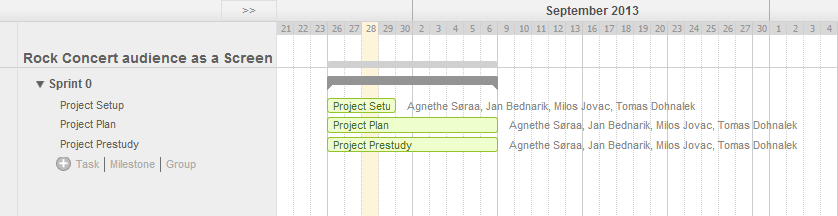
\includegraphics[scale=0.6]{images/gantt}
    \caption{Gantt Chart}
    \label{img:gantt}
\end{center}
\end{figure}

\subsection{Milestones}
\section{Risk management}

\begin{table*}\centering \ra{1.3}
    \caption{Skills}
    \label{tab:skills}
    \vspace{2mm}
    \begin{tabular}{lcccc}
    \toprule
									
    \midrule
    \textbf{Event                	 } & Someone gets sick  		       & 1     & 2     & 3     \\ 
    \textbf{Consiquence              } & 4       					       & 1     & 1     & 1     \\ 
    \textbf{Possibility				 } & 5         						   & 1     & 4     & 1     \\ 
    \textbf{Risk                     } & 20        						   & 4     & 1     & 4     \\ 
    \textbf{Reactive Measures        } & Other people do more ours || Person can work from home         & 3     & 3     & 3     \\ 
    \textbf{Proactive Measures       } & Free weekends        			   & 3     & 1     & 2     \\ 
    \textbf{Responsible              } & All        					   & 2     & 5     & 1     \\ 
   
    \bottomrule
    \end{tabular}
\end{table*}

\begin{table*}\centering \ra{1.3}
    \caption{Skills}
    \label{tab:skills}
    \vspace{2mm}
    \begin{tabular}{lcccc}
    \toprule
                                & Agnethe   & Tomas & Milos & Jan \\
    \midrule
    \textbf{Leadership                 } & 4         & 1     & 2     & 3     \\ 
    \textbf{Scrum                      } & 4         & 1     & 1     & 1     \\ 
    \textbf{Mobile software development} & 3         & 1     & 4     & 1     \\ 
    \textbf{\LaTeX                     } & 1         & 4     & 1     & 4     \\ 
    \textbf{Network programming        } & 2         & 3     & 3     & 3     \\ 
    \textbf{Image processing           } & 1         & 3     & 1     & 2     \\ 
    \textbf{Java                       } & 3         & 2     & 5     & 1     \\ 
    \textbf{C++                        } & 1         & 4     & 3     & 4     \\ 
    \textbf{Testing                    } & 1         & 4     & 2     & 3     \\
    \bottomrule
    \end{tabular}
\end{table*}


\end{document}
